\chapter{简单网络}\label{cha:content3}

\section{非协作单节点定位网络}\label{section:circle_general}
非协作单节点定位网络的性能描述可以借助一种比较直观的方式,为此引入以下\textbf{信息椭圆}的概念\cite{LimitBound}:
\begin{definition}
信息椭圆是参数空间$\theta$上由费舍尔信息矩阵定义的空间曲面:
\begin{equation}\label{eq:ie}
\bm{x}^{\textrm{T}} \,\bm{I}_{\theta}^{-1}\bm{x}=1,\bm{x}\in \mathbb{R}^{2N}.
\end{equation}
\end{definition}
信息椭圆各个主轴的长度衡量了特征值的大小,代表了该方向的定位精度。
下面研究二维情形下由$I(\bm{p})=\sum \lambda_i \bm{u}_i \bm{u}_i^{\textrm{T}} $决定的信息椭圆的形状,即求$I(\bm{p})$的特征值和特征向量。
将二维向量看成复平面的复数,$I(\bm{p})$看成复平面上的线性算子,作用规则是$I(\bm{p})\bm{x}=\sum \lambda_i (\bm{x}\cdot\bm{u}_i)\bm{u}_i$,其值域仍在复平面内,算子$I(\bm{p})$的特征值$\lambda$和特征向量$\bm{y}$满足$I(\bm{p})\bm{y}=\lambda \bm{y}$。


设$\bm{x}$幅角为$\theta$,$\bm{u}_i$幅角为$\phi_i$,由$I(\bm{p})\bm{x}=\sum \lambda_i (\bm{x}\cdot\bm{u}_i)\bm{u}_i$
可得
\begin{equation}
\sum \lambda_i \cos(\theta-\phi_i)e^{j\phi_i}=\lambda e^{i\theta}.
\end{equation}
利用虚部为0的条件,可以进一步得到:
$\theta,\lambda$满足方程组
\begin{align}\label{eq:fim_eq_1}
\begin{cases}
0&=\sum \lambda_i \sin(2(\theta-\phi_i))\\
\lambda&=\sum \lambda_i \cos^2(\theta-\phi_i).
\end{cases}
\end{align}
下面给出关于矩阵$I(\bm{p})$有两个不同的特征值即信息椭圆非退化的一个充要条件:
\begin{theorem}
(\ref{eq:fim_eq_1})中$\lambda$有两个不同的实根当且仅当
\begin{equation}
\sum (\sin(2\phi_i)\lambda_i)^2+(\cos(2\phi_i)\lambda_i)^2 \neq 0.
\end{equation}
\end{theorem}

\begin{proof}
设$A:=\sum\sin(2\phi_i)\lambda_i,B:=\sum\cos(2\phi_i)\lambda_i$

充分性:若$\sqrt{A^2+B^2} \neq 0$,
设$\cos\phi=\frac{A}{\sqrt{A^2+B^2}},\sin\phi=\frac{A}{\sqrt{A^2+B^2}}$
等式$(\ref{eq:fim_eq_1})$可化为:
\begin{equation}
\cos(2\theta+\phi)=0.
\end{equation}
等式$(\ref{eq:fim_eq_1})$中第2式可化为:
\begin{align}\notag\label{eq:Lambda}
\lambda&=\frac{\sum \lambda_i}{2}+\frac{1}{2}\sqrt{A^2+B^2}\sin(2\theta+\phi)\\
&=\frac{\sum \lambda_i}{2}\pm\frac{1}{2}\sqrt{A^2+B^2}.
\end{align}
由条件$A^2+B^2\neq 0$故有两个不相同的实根。

必要性:反设A=0,B=0,则$\forall \theta$,等式$(\ref{eq:fim_eq_1})$成立,且
等式$(\ref{eq:fim_eq_1})$中第2式化为$\lambda=\frac{\sum \lambda_i}{2}$,只有一个特征根,对应$I(\bm{p})$退化为对角阵,矛盾。
\end{proof}
\begin{remark}

根据式(\ref{eq:Lambda})和(\ref{eq:SPEB_formula}),误差下界为
\begin{align}\notag\label{eq:SPEB_min}
\text{SPEB}&=\frac{1} {\tilde{\lambda_1}}+\frac{1}{\tilde{\lambda_2}}\\
&=\frac{4\sum \lambda_i}{(\sum \lambda_i)^2-(A^2+B^2)}
\end{align}
由此可以看出当$A^2+B^2=0$时误差下界最小,此时$I(\bm{p})$的两个特征值相等,信息椭圆退化为圆。

为进一步验证此结论,我们考虑一仿真情形:在单位正方形顶点部署4个锚点,定位强度量$\lambda_i=2+0.3\times(i-1)$,考虑目标节点的位置在每次定位中服从正方形内的二维均匀分布,仿真1000次后得到的定位误差下界和信息椭圆离心率的关系曲线如图\ref{fig:eccentricity}所示。
\begin{figure}
  \centering
  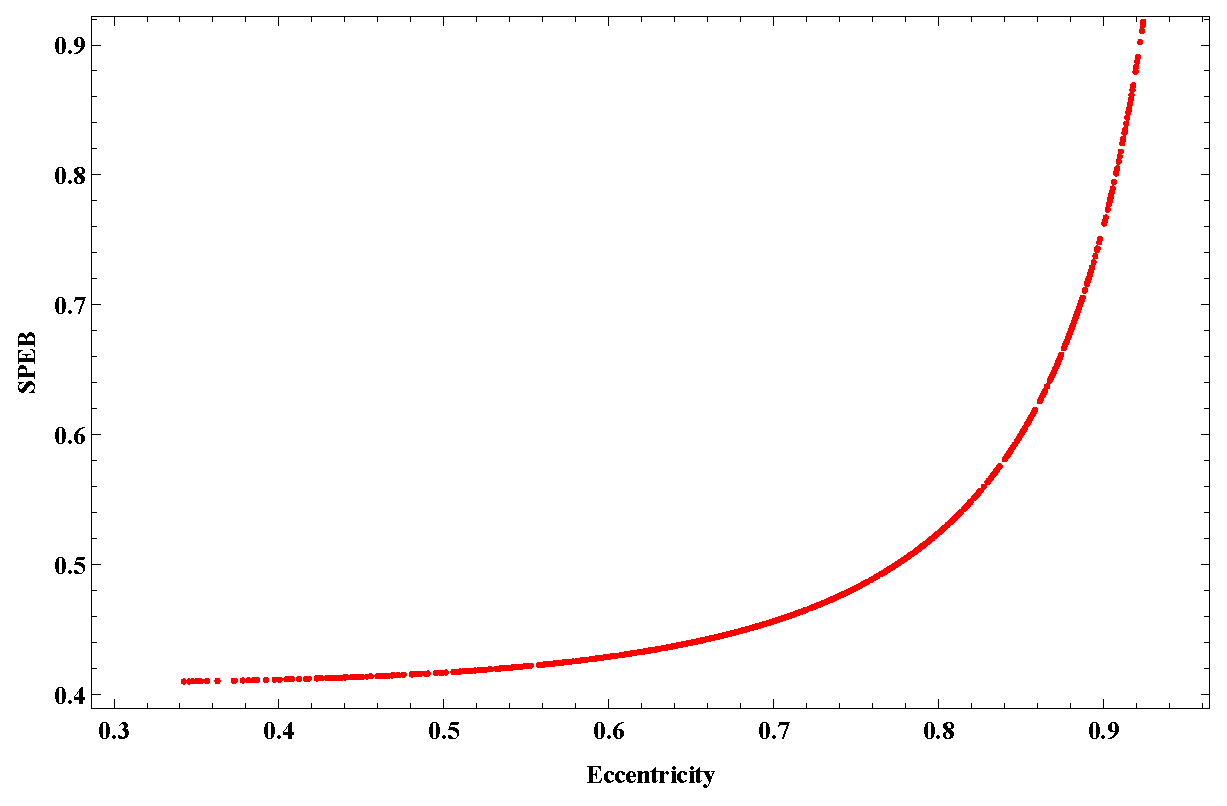
\includegraphics[width=400pt]{eccentricity_SPEB.eps}
  \caption{SPEB与信息椭圆离心率的关系}\label{fig:eccentricity}
\end{figure}
从图\ref{fig:eccentricity}可以看出:
\begin{itemize}
  \item 定位误差下界在$\lambda_i$给定的情况下完全由椭圆离心率决定,如果我们联立$e=\sqrt{1-\lambda_{\min}/\lambda_{\max}}$与式(\ref{eq:Lambda}),式(\ref{eq:SPEB_min})不难得出这个结论
  \item 定位误差下界是椭圆离心率的增函数,这与式(\ref{eq:SPEB_min})相吻合。在椭圆离心率比较小的情况下,误差下界已经接近$e=0$时的$1/\sum \lambda_i=0.408$。
\end{itemize}
\end{remark}
\section{两个未知节点协作的场景}\label{section:two_node_cooperation}
两个移动节点协作情况下,为求4维费舍尔信息矩阵特征多项式的表达式,需要下面的定理:
\begin{theorem}\label{thm:ShenIden}
设$J$是对称正定的矩阵,那么下式成立:
\begin{equation}\label{eq:ShenIden}
|J+\epsilon \bm{u}\bm{u}^{\textrm{T}} |=|J|+\epsilon \bm{u}^{\textrm{T}} J^*\bm{u}
\end{equation}
其中$J^*$表示J的伴随矩阵,满足等式$JJ^*=|J|\bm{I}$。
\end{theorem}
证明上面的定理需要如下两个引理:
\begin{lemma}\cite{aa}\label{lemma:block}
如果方阵$\bm{M}$可以写成分块的形式$\left(\begin{array}{cc}
A&B\\
C&D\\
\end{array}\right)$,而且A是可逆的对角阵,那么$\bm{M}$的行列式$|\bm{M}|=|A||D-CA^{-1}B|$
如果方阵$\bm{M}$可以写成分块的形式$\left(\begin{array}{cc}
A&B\\
C&D\\
\end{array}\right)$,而且A是可逆的对角阵,那么$\bm{M}$的行列式为
\begin{equation}
|\bm{M}|=|A||D-CA^{-1}B|.
\end{equation}
\end{lemma}
\begin{proof}
通过第三类初等变换方阵我们有
\begin{equation}
\left(\begin{array}{cc}
I&0\\
-CA^{-1}&I\\
\end{array}\right) \bm{M}=\left(\begin{array}{cc}
A&B\\
0&D-CA^{-1}B\\
\end{array}\right)
\end{equation}
两边同时取行列式即得要证明的式子。
\end{proof}

\begin{lemma}
如果$\bm{u}$是一个n维的列向量,$\bm{I}$是n维单位阵,则我们有行列式恒等式:
\begin{equation}\label{eq:con_eq}
|(1+\bm{u}^{\textrm{T}} \bm{u})\bm{I}-\bm{u}\bm{u}^{\textrm{T}} |=(1+\bm{u}^{\textrm{T}} \bm{u})^{n-1}.
\end{equation}
\end{lemma}
证明(\ref{eq:con_eq})需要下面的Woodbury 矩阵求逆公式:
\begin{equation}\label{eq:woodbury}
(A+UCV)^{-1}=A^{-1}-A^{-1}U(C^{-1}+VA^{-1}U)^{-1}VA^{-1}
\end{equation}
其中A,C均是可逆的方阵。


\begin{proof}
用数学归纳法证明,首先我们对$n=2$的情形直接验证可得(\ref{eq:con_eq})成立。
假设结论对n-1维的情形成立,设$\bm{u}=(\bm{v}^{\textrm{T}} ,u_n)^{\textrm{T}} $,其中$\bm{v}$是n-1维的列向量,那么对$\bm{v}/\sqrt{1+u_n^2}$用归纳假设有:
\begin{equation}
|(1+\frac{||\bm{v}||^2}{1+u_n^2})\bm{I}_{n-1}-\frac{\bm{v}\bm{v}^{\textrm{T}} }{1+u_n^2}|=(1+\frac{||\bm{v}||^2}{1+u_n^2})^{n-2}
\end{equation}
其中,$||\bm{v}||^2=\bm{v}^{\textrm{T}} \bm{v},||\cdot||$表示欧式空间的2范数。
由上式可得:
\begin{align*}
\begin{cases}
A:&=(1+u_n^2+||\bm{v}||^2)\bm{I}_{n-1}-\bm{v}\bm{v}^{\textrm{T}}\\
|A|&=(1+u_n^2)(1+u_n^2+||\bm{v}||)^{n-2}.
\end{cases}
\end{align*}
对n维的情形,$(1+\bm{u}^{\textrm{T}} \bm{u})\bm{I}-\bm{u}\bm{u}^{\textrm{T}} $可以写成分块矩阵的形式$\left(\begin{array}{cc}
A&-u_n\bm{v}\\
-u_n\bm{v}^{\textrm{T}} &||\bm{v}||^2+1\\
\end{array}\right)$。
由引理(\ref{lemma:block})得:
\begin{equation}\label{eq:LMidd}
|(1+\bm{u}^{\textrm{T}} \bm{u})\bm{I}-\bm{u}\bm{u}^{\textrm{T}} |=|A|(||\bm{v}||^2+1-u_n^2 \bm{v}^{\textrm{T}} A^{-1}\bm{v}).
\end{equation}
由Woodbury矩阵求逆公式:
\begin{equation}\label{eq:AInv}
A^{-1}=\frac{1}{1+||\bm{v}||^2+u_n^2}-\frac{\bm{v}(-1+||\bm{v}||^2/(1+||\bm{v}||^2+u_n^2))^{-1}\bm{v}^{\textrm{T}} }{(1+||\bm{v}||^2+u_n^2)^2}.
\end{equation}
将(\ref{eq:AInv})代入(\ref{eq:LMidd})中,化简即可得对n的情形要证的恒等式成立。
\end{proof}

\begin{proof}[定理(\ref{thm:ShenIden})证明]
式(\ref{eq:ShenIden})等价于:
\begin{equation}\label{eq:ShenIden_1}
|J+\epsilon \bm{u}\bm{u}^{\textrm{T}} |=|J|(1+\epsilon \bm{u}^{\textrm{T}} J^{-1}\bm{u}).
\end{equation}
因为J是对称正定的矩阵,所以存在正交矩阵Q,使得$J=QDQ^{-1}$,D是对角阵,
代入(\ref{eq:ShenIden_1})中得:
$|D+\epsilon \bm{y}\bm{y}^{\textrm{T}} |=|D|(1+\epsilon \bm{y}^{\textrm{T}} D^{-1}\bm{y})$
其中$\bm{y}=Q^{-1}\bm{u}$,因此我们只需对对角矩阵证明定理成立。
设J是n维对角阵,由Woodbury矩阵恒等式可得:
\begin{equation}
(J+\epsilon \bm{u}\bm{u}^{\textrm{T}} )^{-1}=J^{-1}-\frac{1}{\epsilon^{-1}+\bm{u}^{\textrm{T}} J^{-1}\bm{u}}J^{-1}\bm{u}\bm{u}^{\textrm{T}} J^{-1}.
\end{equation}
整理得:
\begin{equation}\label{eq:ShenIden_2}
(J+\epsilon \bm{u}\bm{u}^{\textrm{T}} )^{-1}=J^{-1}\frac{(1+\epsilon\bm{u}^{\textrm{T}} J^{-1}\bm{u})\bm{I}-\epsilon \bm{u}\bm{u}^{\textrm{T}} J^{-1}}{1+\epsilon\bm{u}^{\textrm{T}} J^{-1}\bm{u}}.
\end{equation}
如果我们能证明:
\begin{equation}
|(1+\epsilon\bm{u}^{\textrm{T}} J^{-1}\bm{u})\bm{I}-\epsilon \bm{u}\bm{u}^{\textrm{T}} J^{-1}|=(1+\epsilon\bm{u}^{\textrm{T}} J^{-1}\bm{u})^{n-1}
\end{equation}
则通过对(\ref{eq:ShenIden_2})两边取行列式即可得到要证的式子,这里设$J=\text{diag}(\lambda_1,...\lambda_n)$,取$y=\sqrt{\epsilon}(u_1/\sqrt{\lambda_1},...u_n/\sqrt{\lambda_n})$,那么上式和(\ref{eq:con_eq})具有相同的形式,因此定理结论成立。
\end{proof}
定理(\ref{thm:ShenIden})可以推广为如下一般形式,证明方法同上。
\begin{corollary}设$J$是对称正定的矩阵,则
\begin{equation}
|J+\epsilon \bm{u}\bm{v}^{\textrm{T}} |=|J|+\epsilon \bm{u}^{\textrm{T}} J^*\bm{v}.
\end{equation}
\end{corollary}
下面我们利用定理(\ref{thm:ShenIden})考虑两个节点协作的情形:
原4维FIM结构为:
\begin{equation}
A=\left(\begin{array}{cc}
\bm{\Sigma}_0+\epsilon \bm{u}\bm{u}^{\textrm{T}}  &-\epsilon \bm{u}\bm{u}^{\textrm{T}}  \\
-\epsilon \bm{u}\bm{u}^{\textrm{T}}  & \bm{\Sigma}_1+\epsilon \bm{u}\bm{u}^{\textrm{T}}
\end{array}
\right).
\end{equation}
通过坐标变换将$\bm{\Sigma}_0,\bm{\Sigma}_1$对角化可以得到等价的形式:
\begin{equation}
A=J+\epsilon\binom{\bm{v}}{-\bm{w}}(\bm{v}^{\textrm{T}} ,-\bm{w}^{\textrm{T}} )
\end{equation}
其中$v,w$为单位方向向量,方向角为$\theta$和$\phi$。而J是对角矩阵,第i个对角元为$\lambda_i$,这样特征多项式$|\lambda A-I|=0$就有简单的表达形式:

\begin{equation}\label{eq:4_characteristic_polynomial}
P(\lambda)= (\lambda-a_1)(\lambda-a_2)(\lambda-a_3)(\lambda-a_4)(1+\epsilon(\frac{\cos^2(\theta)}{\lambda-a_1}+
 \frac{\sin^2(\theta)}{\lambda-a_2}+\frac{\cos^2(\phi)}{\lambda-a_3}+\frac{\sin^2(\phi)}{\lambda-a_4})).
\end{equation}
利用SPEB的定义和式(\ref{eq:4_characteristic_polynomial}),可以得到相比于非协作的情形定位误差下界下降的成分为:
\begin{equation}
\Delta=\sum \frac{1}{\lambda_i}-\text{SPEB}_{\text{global}}=\xi\left(\frac{\cos^2(\theta)}{a_1^2}+\frac{\sin^2(\theta)}{a_2^2}+\frac{\cos^2(\phi)}{a_3^2}+\frac{\sin^2(\phi)}{a_4^2}\right)
\end{equation}
其中
\begin{equation}
\xi=\left(\frac{1}{\epsilon}+\frac{\cos^2(\phi)}{a_3}+\frac{\sin^2(\phi)}{a_4}+\frac{\cos^2(\theta)}{a_1}+\frac{\sin^2(\theta)}{a_2}\right)^{-1}.
\end{equation}
考察上面关于$\theta$和$\phi$的函数,我们有如下定理,推导过程见附录[\ref{B_F_0}]:
\begin{theorem}\label{theorem:2node_in_cooperation}
如果$\frac{1}{a_1}+\frac{1}{a_2}\geq \max\{\frac{1}{a_4},\frac{1}{a_3}\}$且$\frac{1}{a_3}+\frac{1}{a_4}\geq\max\{\frac{1}{a_1},\frac{1}{a_2}\}$,那么$\theta=\phi=\frac{\pi}{2}$是$\Delta$的最大值点。
\end{theorem}
\section{本章小结}\label{section:conclusion3}
  % Keep the summary *very short*.
  我们在本章中针对简单网络研究了通过改变角度参数使得误差下界最小这一问题,现总结如下:
  \begin{itemize}
  \item 对于非协作情形,如果能改变锚点部署的角度使得费舍尔信息矩阵是对角阵(信息椭圆退化成圆),则误差下界最小,但根据图\ref{fig:eccentricity}的结果,仿真1000次大部分情况下椭圆离心率在0.4以上,因此信息椭圆退化成圆只是一个理论最优的结果,实际系统很难达到。
  \item 对于两节点协作的情形,定理\ref{theorem:2node_in_cooperation}给出了一个充分条件以确定定位误差最小的情形。
  \end{itemize}


  尽管锚点贡献的信息椭圆在实际中很难退化成圆,但从\ref{section:two_node_cooperation}小节的推导来看,锚点贡献的信息是各向异性的情况下作理论推导会非常困难,文献\cite{LimitBound3}给出了三个节点协作场景下定位误差下界一般的表达式,但对于更多节点协作的情形,如果我们关心协作信息的特性,不妨简化锚点贡献的信息为各向同性的,这样做一方面是出于进一步理论分析的方便同时又不影响要研究的主要问题。
  因此在接下来的研究中,我们总是假设式(\ref{eq:general_fim})中出现的$I(\bm{p}_i)$是形如$c\bm{I}_2$的对角阵。
  在接下来的研究工作中我们会采用不同于\ref{section:two_node_cooperation}小节的数学方法来求解费舍尔信息矩阵的特征值。
